\documentclass[]{article}
\usepackage{lmodern}
\usepackage{amssymb,amsmath}
\usepackage{ifxetex,ifluatex}
\usepackage{fixltx2e} % provides \textsubscript
\ifnum 0\ifxetex 1\fi\ifluatex 1\fi=0 % if pdftex
  \usepackage[T1]{fontenc}
  \usepackage[utf8]{inputenc}
\else % if luatex or xelatex
  \ifxetex
    \usepackage{mathspec}
  \else
    \usepackage{fontspec}
  \fi
  \defaultfontfeatures{Ligatures=TeX,Scale=MatchLowercase}
\fi
% use upquote if available, for straight quotes in verbatim environments
\IfFileExists{upquote.sty}{\usepackage{upquote}}{}
% use microtype if available
\IfFileExists{microtype.sty}{%
\usepackage{microtype}
\UseMicrotypeSet[protrusion]{basicmath} % disable protrusion for tt fonts
}{}
\usepackage[margin=1in]{geometry}
\usepackage{hyperref}
\hypersetup{unicode=true,
            pdftitle={Warfarin Dosing Service Analysis},
            pdfauthor={Brian Gulbis, PharmD, BCPS},
            pdfborder={0 0 0},
            breaklinks=true}
\urlstyle{same}  % don't use monospace font for urls
\usepackage{longtable,booktabs}
\usepackage{graphicx,grffile}
\makeatletter
\def\maxwidth{\ifdim\Gin@nat@width>\linewidth\linewidth\else\Gin@nat@width\fi}
\def\maxheight{\ifdim\Gin@nat@height>\textheight\textheight\else\Gin@nat@height\fi}
\makeatother
% Scale images if necessary, so that they will not overflow the page
% margins by default, and it is still possible to overwrite the defaults
% using explicit options in \includegraphics[width, height, ...]{}
\setkeys{Gin}{width=\maxwidth,height=\maxheight,keepaspectratio}
\IfFileExists{parskip.sty}{%
\usepackage{parskip}
}{% else
\setlength{\parindent}{0pt}
\setlength{\parskip}{6pt plus 2pt minus 1pt}
}
\setlength{\emergencystretch}{3em}  % prevent overfull lines
\providecommand{\tightlist}{%
  \setlength{\itemsep}{0pt}\setlength{\parskip}{0pt}}
\setcounter{secnumdepth}{0}
% Redefines (sub)paragraphs to behave more like sections
\ifx\paragraph\undefined\else
\let\oldparagraph\paragraph
\renewcommand{\paragraph}[1]{\oldparagraph{#1}\mbox{}}
\fi
\ifx\subparagraph\undefined\else
\let\oldsubparagraph\subparagraph
\renewcommand{\subparagraph}[1]{\oldsubparagraph{#1}\mbox{}}
\fi
\usepackage{float}

%%% Use protect on footnotes to avoid problems with footnotes in titles
\let\rmarkdownfootnote\footnote%
\def\footnote{\protect\rmarkdownfootnote}

%%% Change title format to be more compact
\usepackage{titling}

% Create subtitle command for use in maketitle
\newcommand{\subtitle}[1]{
  \posttitle{
    \begin{center}\large#1\end{center}
    }
}

\setlength{\droptitle}{-2em}
  \title{Warfarin Dosing Service Analysis}
  \pretitle{\vspace{\droptitle}\centering\huge}
  \posttitle{\par}
\subtitle{Department of Pharmacy Services - Memorial Hermann-Texas Medical Center}
  \author{Brian Gulbis, PharmD, BCPS}
  \preauthor{\centering\large\emph}
  \postauthor{\par}
  \predate{\centering\large\emph}
  \postdate{\par}
  \date{January 2015 to December 2015}

\begin{document}
\maketitle

\subsection{Service Utilization}\label{service-utilization}

\subsubsection{Annual Warfarin
Utilization}\label{annual-warfarin-utilization}

The number of patients receiving warfarin while at Memorial
Hermann-Texas Medical Center continues to increase annually (see figure
1).

\begin{figure}[H]
\centering
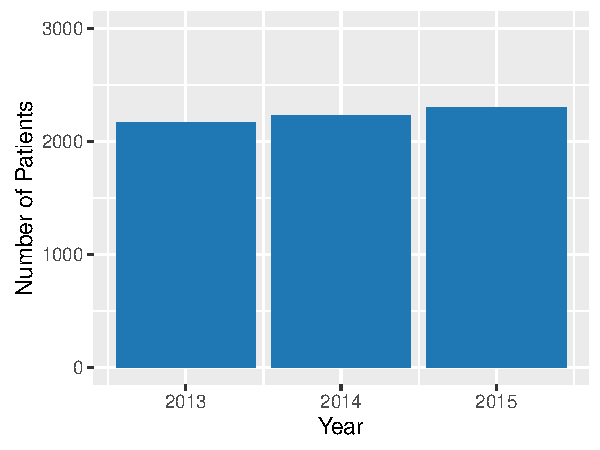
\includegraphics{warfarin_analysis_2015_files/figure-latex/graph_utilization-1.pdf}
\caption{Number of Patients Receiving Warfarin at MH-TMC, 2013-2015}
\end{figure}

\subsubsection{Utilization of Pharmacy Dosing
Service}\label{utilization-of-pharmacy-dosing-service}

Utilization of the Pharmacy Dosing Service continues to increase on an
annual basis (see figure 2). The Pharmacy Dosing Service is responsible
for managing approximately 60\% of the daily warfarin doses ordered in
the hospital (see figure 3). The remainder of the doses are ordered by
traditional health care providers, including physicians, nurse
practitioners, and physician assistants. Many of the warfarin doses in
the traditional group are ordered in consultation with a clinical
pharmacist or clinical pharmacist-specialist, and all warfarin doses are
reviewed and verified by a pharmacist.

\begin{figure}[H]
\centering
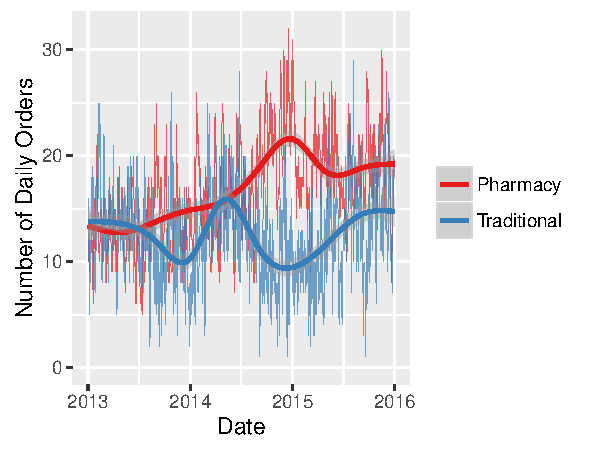
\includegraphics{warfarin_analysis_2015_files/figure-latex/dose_service_use-1.pdf}
\caption{Daily Warfarin Orders Managed by Pharmacy and Traditional}
\end{figure}

\begin{figure}[H]
\centering
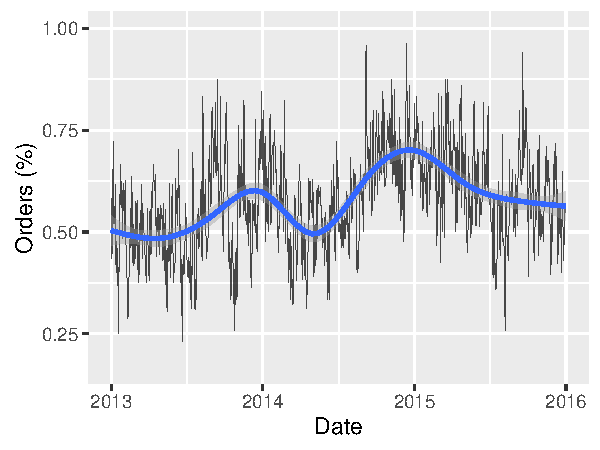
\includegraphics{warfarin_analysis_2015_files/figure-latex/dose_service_use2-1.pdf}
\caption{Percent of Daily Warfarin Orders Managed by Pharmacy Dosing
Service}
\end{figure}

The medical services with the largest number of patients on warfarin
include Cardiology and Internal Medicine. Utilization of the Pharmacy
Dosing Service remains low among patients on the Cardiology services
(see figure 4).

\begin{figure}[H]
\centering
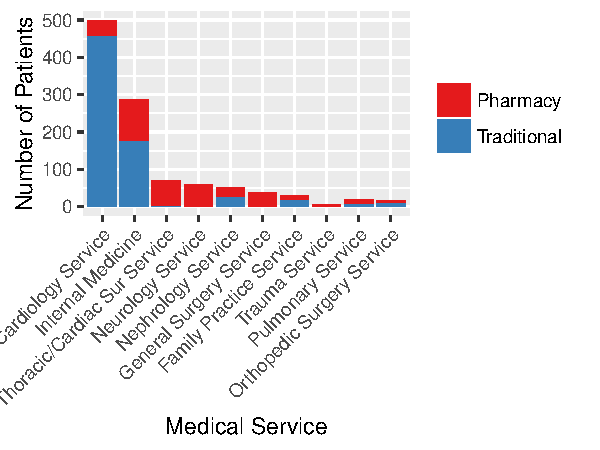
\includegraphics{warfarin_analysis_2015_files/figure-latex/ds_med_service_curr-1.pdf}
\caption{Pharmacy Dosing Service Utilization Among Top 10 Medical
Services Ordering Warfarin}
\end{figure}

\subsection{Comparison}\label{comparison}

The efficacy and safety of patients whose warfarin therapy was managed
by the Pharmacy Dosing Service was compared with those patients whose
warfarin therapy was managed by traditional health care providers.
Patients were assigned to each group and included or excluded from the
analysis using the following criteria:

\begin{itemize}
\tightlist
\item
  Group 1 - Pharmacy Dosing Service

  \begin{itemize}
  \tightlist
  \item
    Consult placed within 48 hours of warfarin initiation
  \item
    At least 60\% of warfarin doses placed by pharmacist
  \end{itemize}
\item
  Group 2 - Traditional Dosing
\end{itemize}

\paragraph{Inclusion}\label{inclusion}

\begin{itemize}
\tightlist
\item
  January 1, 2015 to December 31, 2015
\item
  Age 18 years or greater
\item
  Received at least 3 doses of warfarin
\item
  Baseline INR \textless{} 1.5
\end{itemize}

\paragraph{Exclusion}\label{exclusion}

\begin{itemize}
\tightlist
\item
  Concurrent DTI or TSOAC
\item
  Liver dysfunction

  \begin{itemize}
  \tightlist
  \item
    AST and ALT \textgreater{} 5x ULN (concurrently)
  \item
    ALT \textgreater{} 10x ULN
  \item
    T.Bili \textgreater{} 3x ULN
  \end{itemize}
\item
  Missing goals of therapy data
\item
  Readmission encounters
\end{itemize}

\subsubsection{Results}\label{results}

This analysis of warfarin patients for 2015 marks the first time that
there were a larger number of patients in the Pharmacy Dosing Service
arm than in the Traditional arm (see Table 1). Patients in the Pharmacy
Dosing Service arm tended to be younger than in the Traditional arm.
Additionally, there were a larger percent patients who were new to
warfarin therapy in the Pharmacy Dosing Service arm.

\begin{longtable}[]{@{}llll@{}}
\caption{Demographics}\tabularnewline
\toprule
& pharmacy & traditional & p\tabularnewline
\midrule
\endfirsthead
\toprule
& pharmacy & traditional & p\tabularnewline
\midrule
\endhead
n & 402 & 285 &\tabularnewline
Age (median {[}IQR{]}) & 58.00 {[}42.25, 68.75{]} & 64.00 {[}54.00,
72.00{]} & \textless{}0.001\tabularnewline
Sex = Male (\%) & 240 (59.7) & 182 (64.1) & 0.279\tabularnewline
BMI (median {[}IQR{]}) & 28.48 {[}24.40, 33.54{]} & 29.32 {[}25.18,
33.68{]} & 0.277\tabularnewline
Race (\%) & & & 0.096\tabularnewline
- African American & 104 (28.4) & 74 (27.9) &\tabularnewline
- Asian & 12 ( 3.3) & 1 ( 0.4) &\tabularnewline
- Native Am. & 0 ( 0.0) & 1 ( 0.4) &\tabularnewline
- Other & 78 (21.3) & 59 (22.3) &\tabularnewline
- White/Caucasian & 172 (47.0) & 130 (49.1) &\tabularnewline
Length of Stay (median {[}IQR{]}) & 12.10 {[}7.71, 19.83{]} & 13.71
{[}8.04, 24.17{]} & 0.103\tabularnewline
Therapy = New/Previous (\%) & 270/132 (67.2/32.8) & 143/142 (50.2/49.8)
& \textless{}0.001\tabularnewline
\bottomrule
\end{longtable}

There were a larger percent of patients with DVT and PE managed by the
Pharmacy Dosing Service, while a larger percent of patients in the
Traditional arm had Atrial Fibrillation (see figure 5). There were no
patients with Ventricular Assist Devices in the Pharmacy Dosing Service
arm, however, this is one example of an area included in the Traditional
group where the clinical pharmacist-specialists are highly involved in
the daily management of warfarin through collaboration with the health
care team.

\begin{figure}[H]
\centering
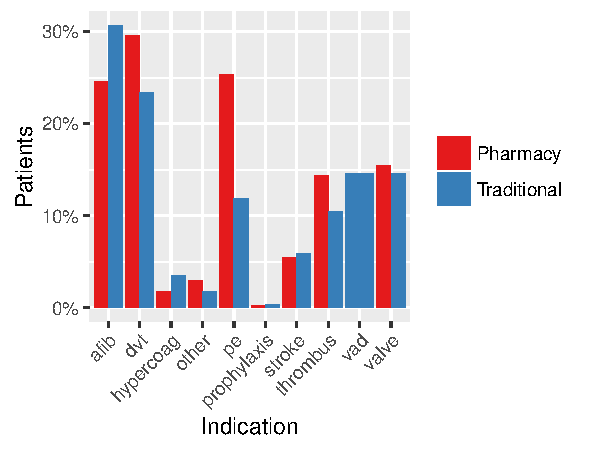
\includegraphics{warfarin_analysis_2015_files/figure-latex/indications-1.pdf}
\caption{Indications for warfarin use}
\end{figure}

There were small differences in the discharge disposition of patients in
each of the two groups, although this likely is not clinically
significant (see figure 6).

\begin{figure}[H]
\centering
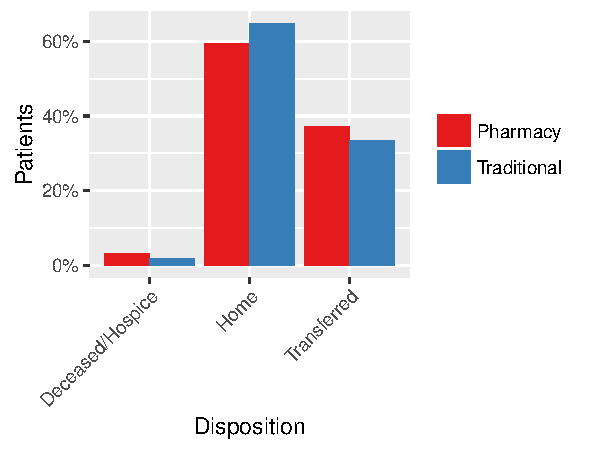
\includegraphics{warfarin_analysis_2015_files/figure-latex/disposition-1.pdf}
\caption{Disposition on discharge}
\end{figure}

The median number of days that patients received warfarin while in the
hospital was lower in the Pharmacy Dosing Service arm compared with the
Traditional arm (5 vs.~6 days, respectively; see figure 7).

\begin{figure}[H]
\centering
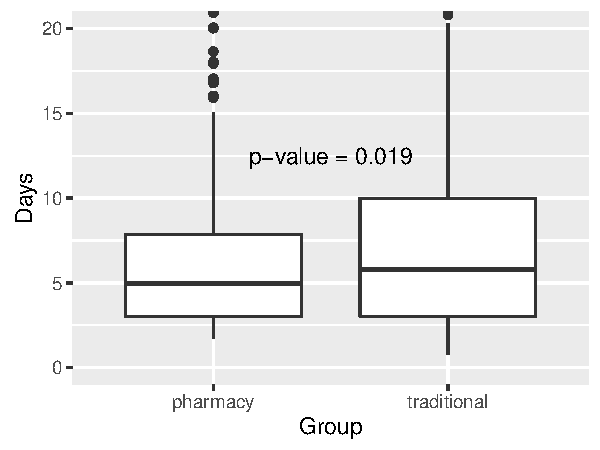
\includegraphics{warfarin_analysis_2015_files/figure-latex/dosing_days-1.pdf}
\caption{Inpatient Dosing Days}
\end{figure}

\subsubsection{Efficacy Endpoints}\label{efficacy-endpoints}

There was a small but statistically significant greater increase in the
INR in patients managed by the Pharmacy Dosing Service compared with the
Traditional arm (see figures 8 and 9).

\begin{figure}[H]
\centering
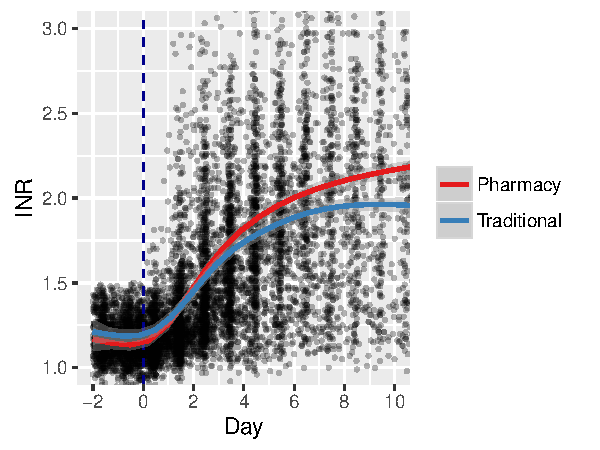
\includegraphics{warfarin_analysis_2015_files/figure-latex/inr-1.pdf}
\caption{INR response after starting warfarin}
\end{figure}

\begin{figure}[H]
\centering
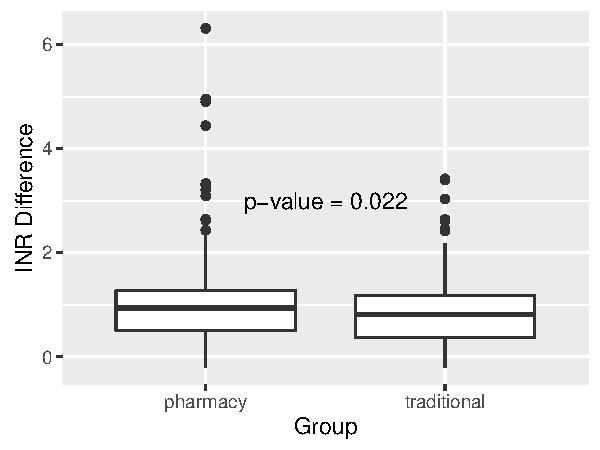
\includegraphics{warfarin_analysis_2015_files/figure-latex/inr2-1.pdf}
\caption{Change in INR}
\end{figure}

The percent of time the INR was in the therapeutic range was similar
between the two groups (see figure 10).

\begin{figure}[H]
\centering
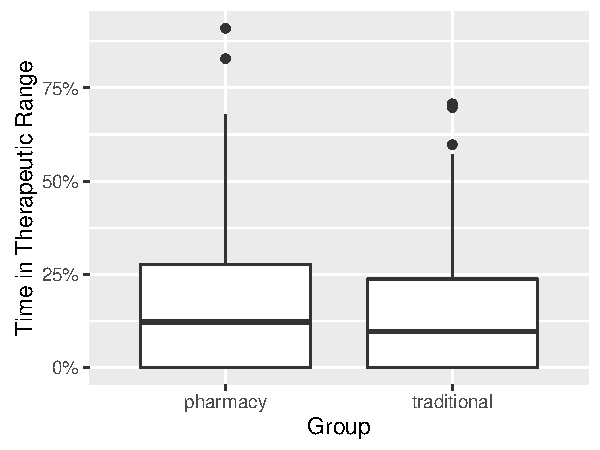
\includegraphics{warfarin_analysis_2015_files/figure-latex/ttr-1.pdf}
\caption{Percent of time INR is within therapeutic range}
\end{figure}

\subsubsection{Safety Endpoints}\label{safety-endpoints}

With the exception of a few outlier patients, the percent of time the
INR was critical (defined as an INR \textgreater{}/= 4) was very small
(median \textless{} 0.00001\% in both groups; see figure 11).

\begin{figure}[H]
\centering
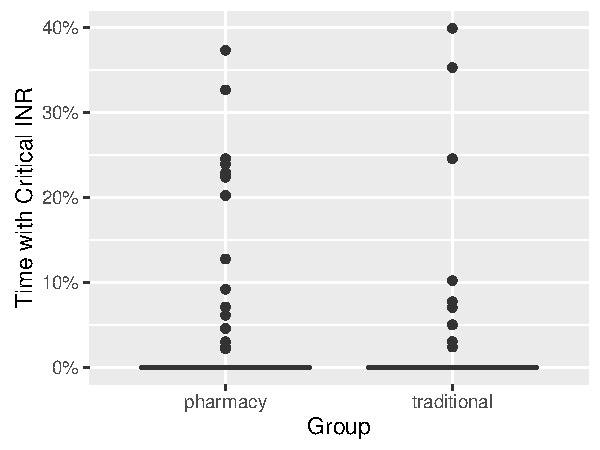
\includegraphics{warfarin_analysis_2015_files/figure-latex/time_above4-1.pdf}
\caption{Percent of time INR is critical (at or above 4)}
\end{figure}

There was a trend towards a greater decrease in the hemoglobin in the
Traditional group compared with the Pharmacy Dosing Service, although
the difference did not reach statistical significance (see figures 12
and 13).

\begin{figure}[H]
\centering
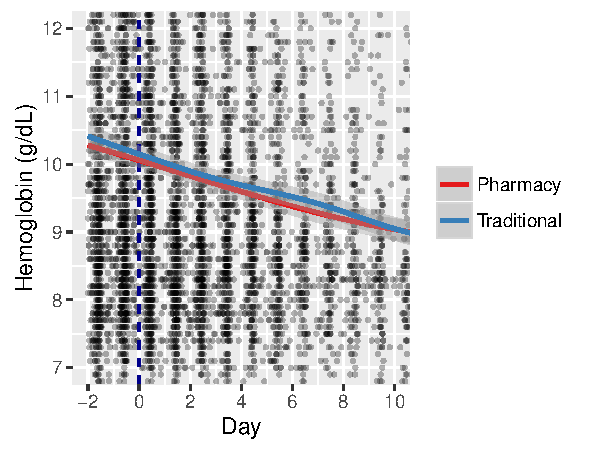
\includegraphics{warfarin_analysis_2015_files/figure-latex/hgb-1.pdf}
\caption{Change in hemoglobin after starting warfarin}
\end{figure}

\begin{figure}[H]
\centering
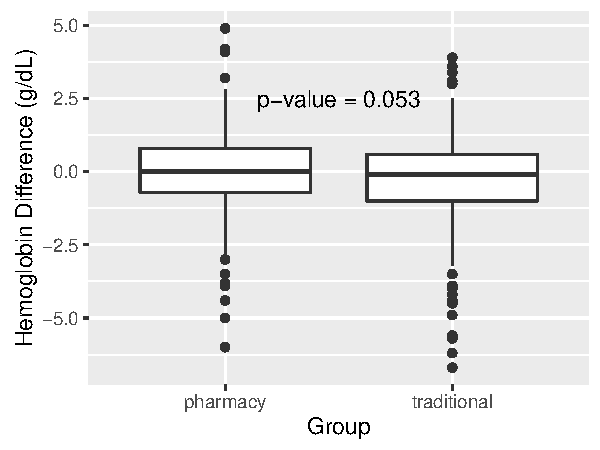
\includegraphics{warfarin_analysis_2015_files/figure-latex/hgb2-1.pdf}
\caption{Change in Hemoglobin}
\end{figure}

\subsection{Historical Comparison}\label{historical-comparison}

A secondary analysis was performed, comparing the Pharmacy Dosing
Service against itself (2015 vs.~2013 to 2014). The same inclusion and
exclusion criteria were used. Patient demographics were similar between
the two groups, except for a slightly younger median age in the 2015
group (see Table 2).

\begin{longtable}[]{@{}llll@{}}
\caption{Demographics}\tabularnewline
\toprule
& current & historical & p\tabularnewline
\midrule
\endfirsthead
\toprule
& current & historical & p\tabularnewline
\midrule
\endhead
n & 402 & 866 &\tabularnewline
Age (median {[}IQR{]}) & 58.00 {[}42.25, 68.75{]} & 59.00 {[}46.00,
71.00{]} & 0.048\tabularnewline
Sex = Male (\%) & 240 (59.7) & 505 (58.3) & 0.685\tabularnewline
BMI (mean (sd)) & 29.95 (8.50) & 29.90 (9.26) & 0.926\tabularnewline
Race (\%) & & & 0.189\tabularnewline
- African American & 104 (28.4) & 245 (31.2) &\tabularnewline
- Asian & 12 ( 3.3) & 15 ( 1.9) &\tabularnewline
- Latin American & 0 ( 0.0) & 1 ( 0.1) &\tabularnewline
- Other & 78 (21.3) & 133 (16.9) &\tabularnewline
- White/Caucasian & 172 (47.0) & 392 (49.9) &\tabularnewline
-Length of Stay (median {[}IQR{]}) & 12.10 {[}7.71, 19.83{]} & 11.85
{[}7.38, 18.62{]} & 0.172\tabularnewline
Therapy = New/Previous (\%) & 270/132 (67.2/32.8) & 604/262 (69.7/30.3)
& 0.390\tabularnewline
\bottomrule
\end{longtable}

Among the medical services which utilize warfarin the most, there was a
slight increase in number of Pharmacy Dosing Serivce patients on the
Cardiology service in 2015 and a slight decrease in patients on Internal
Medicine (see figure 14).

\begin{figure}[H]
\centering
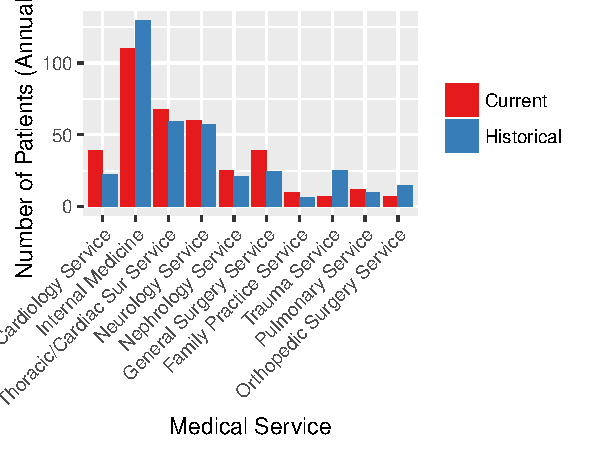
\includegraphics{warfarin_analysis_2015_files/figure-latex/ds_med_service-1.pdf}
\caption{Pharmacy Dosing Service Utilization Among Top 10 Medical
Services Ordering Warfarin}
\end{figure}

The indications for anticoagulation remain relatively unchanged from
2013-2014 to 2015 (see figure 15), as do the discharge dispositions (see
figure 16).

\begin{figure}[H]
\centering
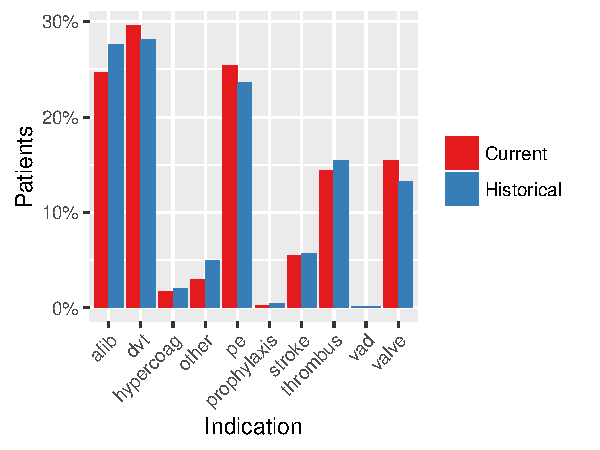
\includegraphics{warfarin_analysis_2015_files/figure-latex/indications_hist-1.pdf}
\caption{Indications for warfarin use}
\end{figure}

\begin{figure}[H]
\centering
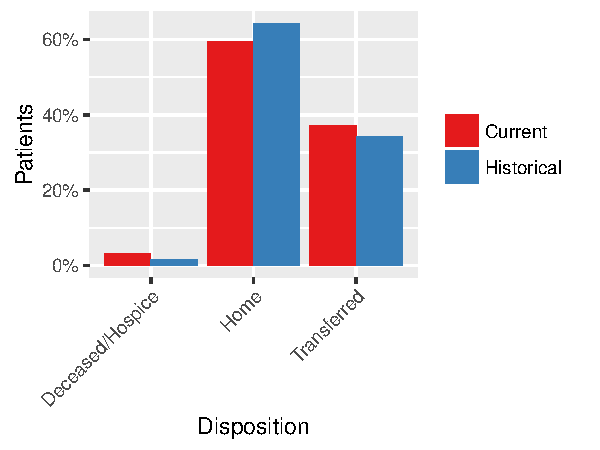
\includegraphics{warfarin_analysis_2015_files/figure-latex/disposition_hist-1.pdf}
\caption{Disposition on discharge}
\end{figure}

The median number of days that patients received warfarin while in the
hospital remains unchanged from 2013-2014 to 2015 (see figure 17).

\begin{figure}[H]
\centering
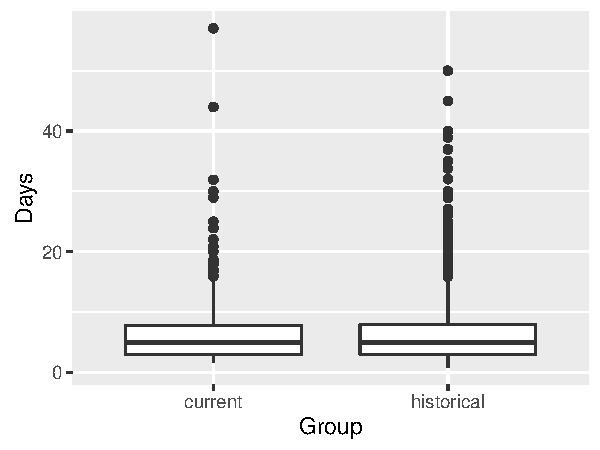
\includegraphics{warfarin_analysis_2015_files/figure-latex/dosing_days_hist-1.pdf}
\caption{Inpatient Dosing Days}
\end{figure}

\subsubsection{Efficacy Endpoints}\label{efficacy-endpoints-1}

The increase in INR was similar between the 2013-2014 and 2015 groups
(see figures 18 and 19).

\begin{figure}[H]
\centering
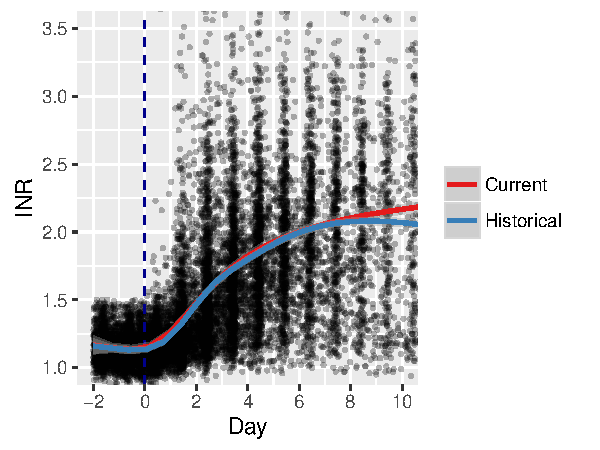
\includegraphics{warfarin_analysis_2015_files/figure-latex/inr_hist-1.pdf}
\caption{Change in INR after starting warfarin}
\end{figure}

\begin{figure}[H]
\centering
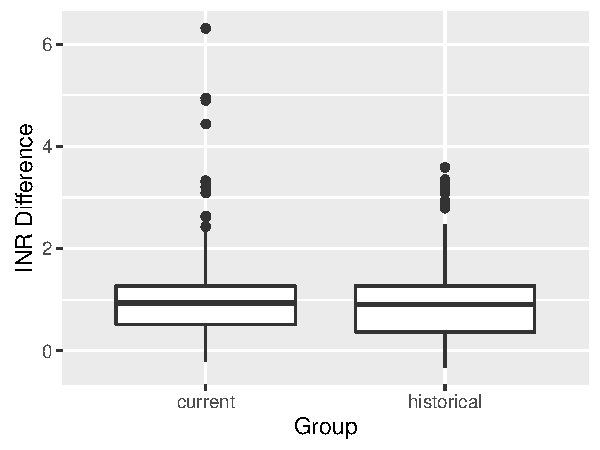
\includegraphics{warfarin_analysis_2015_files/figure-latex/inr2_hist-1.pdf}
\caption{Change in INR}
\end{figure}

The median percent of time the INR was within the therapeutic range
increased slightly in 2015 compared with 2013-2014, although the
difference was not statistically significant (see figure 20).

\begin{figure}[H]
\centering
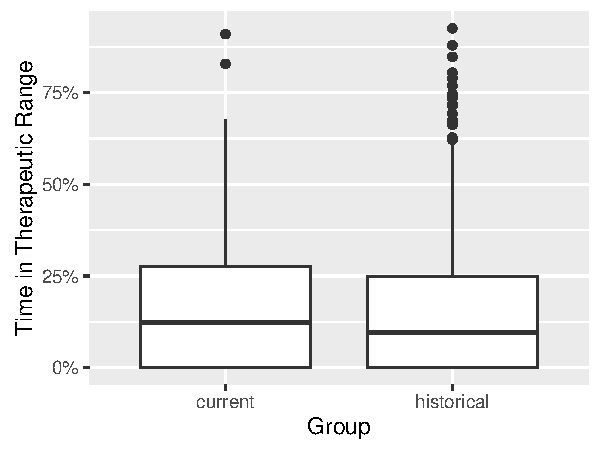
\includegraphics{warfarin_analysis_2015_files/figure-latex/ttr_hist-1.pdf}
\caption{Percent of time INR is within therapeutic range}
\end{figure}

\subsubsection{Safety Endpoints}\label{safety-endpoints-1}

The median percent of time the INR was critical remains very low in both
2013-2014 and 2015 (see figure 21).

\begin{figure}[H]
\centering
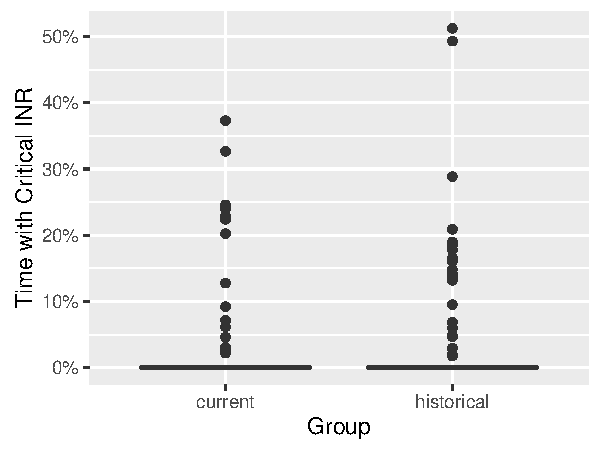
\includegraphics{warfarin_analysis_2015_files/figure-latex/critical_hist-1.pdf}
\caption{Percent of time INR is critical (at or above 4)}
\end{figure}

There was a trend towards less of a decrease in the hemoglobin in 2015
compared with 2013-2014, although the difference did not reach
statistical significance (see figures 22 and 23).

\begin{figure}[H]
\centering
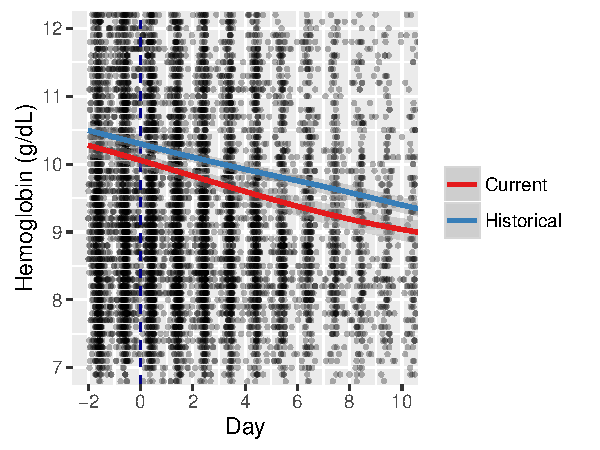
\includegraphics{warfarin_analysis_2015_files/figure-latex/hgb_hist-1.pdf}
\caption{Change in hemoglobin after starting warfarin}
\end{figure}

\begin{figure}[H]
\centering
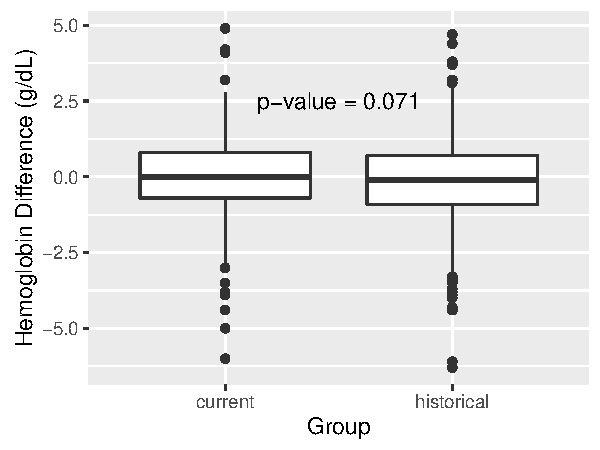
\includegraphics{warfarin_analysis_2015_files/figure-latex/hgb2_hist-1.pdf}
\caption{Change in Hemoglobin}
\end{figure}

\subsection{Conclusions}\label{conclusions}

\begin{itemize}
\tightlist
\item
  Utilization of the Pharmacy Dosing Service continues to increase.
\item
  Patients managed by the Pharmacy Dosing Service had a larger increase
  in the INR compared with Traditional management.
\item
  There was a trend towards a larger decrease in the hemoglobin in
  patients in the Traditional group compared with the Pharmacy Dosing
  Service.
\item
  There were no major differences in efficacy or safety outcomes when
  comparing patients managed by the Pharmacy Dosing Service in 2013-2014
  with 2015.
\end{itemize}

\subsection{Statistical Analysis}\label{statistical-analysis}

Data preparation and statistical analysis were performed using R version
3.3.1 (2016-06-21) on a windows x64 system.

\paragraph{Reference}\label{reference}

R Core Team (2016). R: A language and environment for statistical
computing. R Foundation for Statistical Computing, Vienna, Austria. URL
\url{https://www.R-project.org/}.

\end{document}
